
\documentclass[12pt]{article}
\topmargin=-1.0cm
\textheight=23cm
\evensidemargin=-1.0cm
\oddsidemargin=-1.0cm
\textwidth=19cm



% TikZ - TikZ ist kein Zeichenprogramm:
\usepackage{tikz}
%\usetikzlibrary{calc}                 % maybe later
\usetikzlibrary{positioning}
\usetikzlibrary{arrows,intersections}

% PGF - Portable Graphics File:


% To define custom colors in plots - must appear after \usepackage{tikz}
\usepackage{color}
\definecolor{mygreen}{rgb}{0,0.6,0}
%\definecolor{mygray}{rgb}{0.5,0.5,0.5}
%\definecolor{mymauve}{rgb}{0.58,0,0.82}


\begin{document}

\title{Demo Plots with TikZ and PGF}
%\subtitle{(A Grab-Bag of Copy-And-Paste Recipes)}  % error!
\author{Robin Schmidt}
\maketitle

%===================================================================================================
\section{With TikZ Only}

%---------------------------------------------------------------------------------------------------
\subsection{Monomials}

\begin{figure}[h]
\centering
\caption{Monomials of degrees $0$ to $5$}
\label{Fig:Monomials}
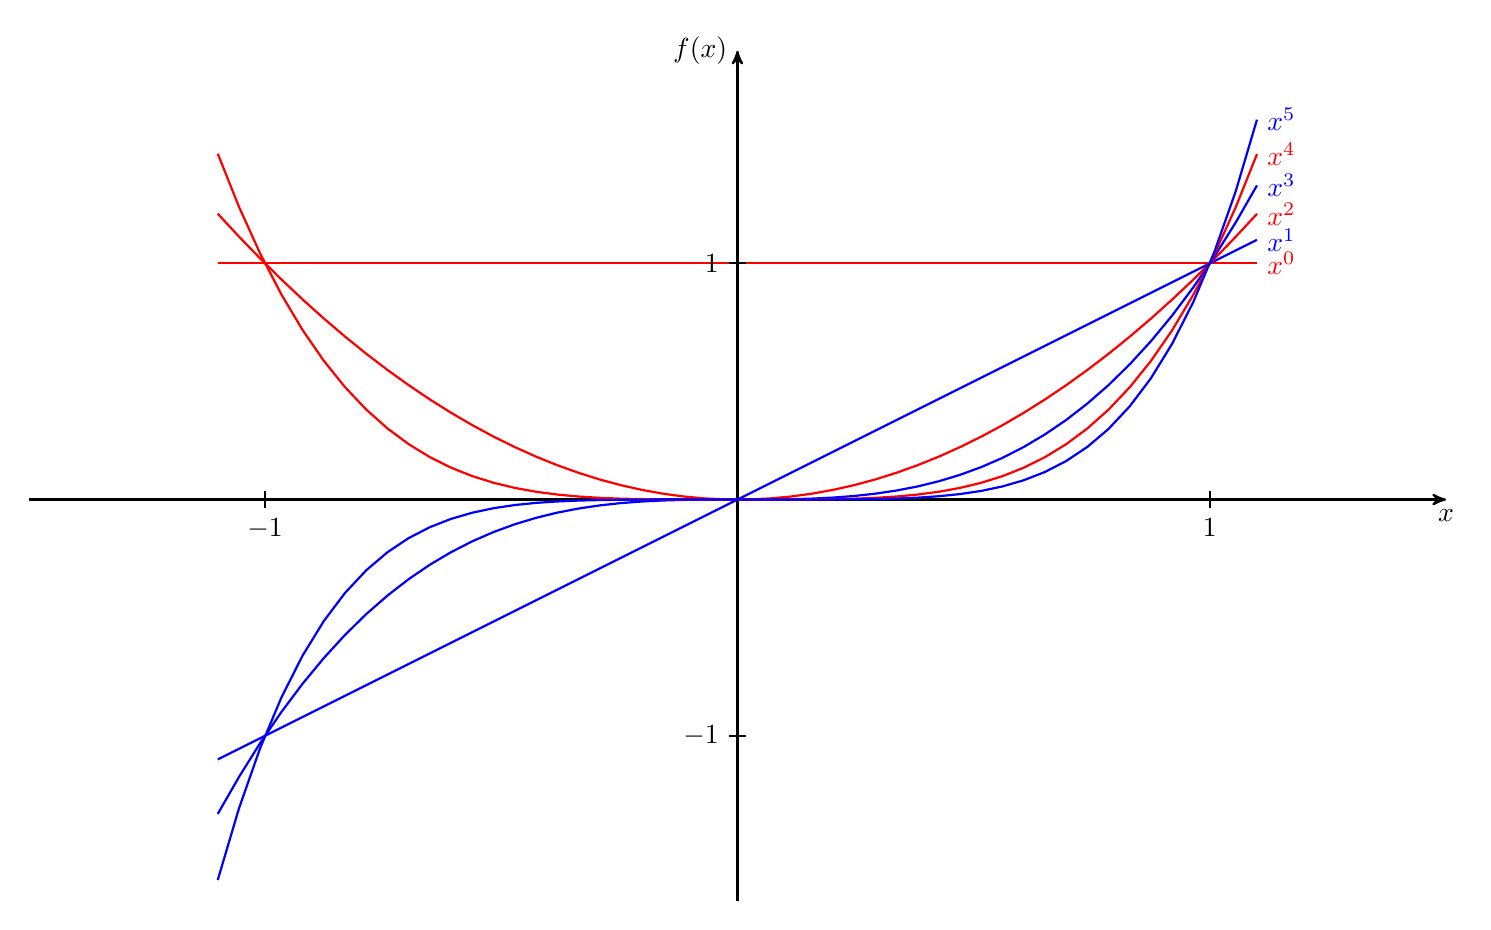
\begin{tikzpicture}
[domain=-1.1:1.1, range=-1.2:1.2, xscale=6, yscale=3, samples=50, thick, >=stealth']

% Coordinate axes:
\draw[->] (-1.5,0) -- (1.5,0) node[below] {$x$};
\draw[->] (0,-1.7) -- (0,1.9) node[left]  {$f(x)$};

% Graphs:
\draw[color=red]  plot (\x,{pow(\x,0)}) node[right] {$x^0$};
\draw[color=blue] plot (\x,{pow(\x,1)}) node[right] {$x^1$};
\draw[color=red]  plot (\x,{pow(\x,2)}) node[right] {$x^2$};
\draw[color=blue] plot (\x,{pow(\x,3)}) node[right] {$x^3$};
\draw[color=red]  plot (\x,{pow(\x,4)}) node[right] {$x^4$};
\draw[color=blue] plot (\x,{pow(\x,5)}) node[right] {$x^5$};

% Tick marks on x-axis:
\draw [shift={(-1,0)}] (0pt,+1pt) -- (0pt,-1pt) node [below] {$-1$};  
\draw [shift={( 1,0)}] (0pt,+1pt) -- (0pt,-1pt) node [below] {$1$};
% The point size 1pt results from 3 / yscale

% Tick marks on y-axis:
\draw [shift={(0,1)}]  (+.5pt, 0pt) -- (-.5pt, 0pt) node [left] {$1$};
\draw [shift={(0,-1)}] (+.5pt, 0pt) -- (-.5pt, 0pt) node [left] {$-1$};
% The point size .5pt results from 3 / xscale

\end{tikzpicture}
\end{figure}

%---------------------------------------------------------------------------------------------------
\subsection{Sine and Cosine}

\begin{figure}[h]
\centering
\caption{Sine and cosine function}
\label{Fig:SineAndCosine}
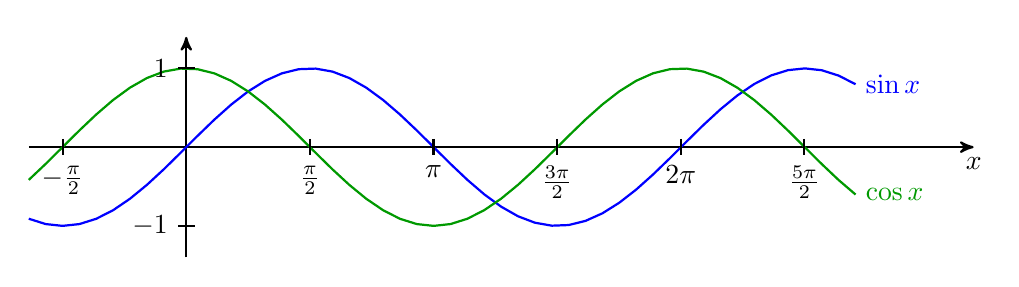
\begin{tikzpicture}
[domain=-2:8.5, samples=50, thick, >=stealth']

% Coordinate axes:
\draw[->] (-2.0,0) -- (10.0,0) node[below] {$x$};
\draw[->] (0,-1.4) -- (0,1.4) node[left]  {};

% Graphs of sin(x) and cos(x):
\draw[color=blue] plot (\x,{sin(\x r)}) node[right] {$\sin x$};
\draw[color=mygreen]  plot (\x,{cos(\x r)}) node[right] {$\cos x$};
% \x r means to convert '\x' from degrees to radians
  
% Tick marks on x-axis:
\draw [shift={(-1.57,0)}] (0pt,+3pt) -- (0pt,-3pt) node [below] {$-\frac{\pi}{2}$};  
\draw [shift={( 1.57,0)}] (0pt,+3pt) -- (0pt,-3pt) node [below] {$\frac{\pi}{2}$};
\draw [shift={( 3.14,0)}] (0pt,+3pt) -- (0pt,-3pt) node [below] {$\pi$};
\draw [shift={( 4.71,0)}] (0pt,+3pt) -- (0pt,-3pt) node [below] {$\frac{3\pi}{2}$};
\draw [shift={( 6.28,0)}] (0pt,+3pt) -- (0pt,-3pt) node [below] {$2\pi$};
\draw [shift={( 7.85,0)}] (0pt,+3pt) -- (0pt,-3pt) node [below] {$\frac{5\pi}{2}$};  
  
% Tick marks on y-axis:
\draw [shift={(0,1)}]  (+3pt, 0pt) -- (-3pt, 0pt) node [left] {$1$};
\draw [shift={(0,-1)}] (+3pt, 0pt) -- (-3pt, 0pt) node [left] {$-1$};
    
\end{tikzpicture}
\end{figure}



\end{document}